\documentclass{beamer}

%--% Paquetes %----------------------------------%
\usepackage[spanish]{babel}
\usepackage[utf8]{inputenc}
\usepackage[T1]{fontenc}
\usepackage{graphicx}
\usepackage{hyperref}
\usepackage{courier}
\usepackage{listings}
\usepackage{xcolor}
\usepackage{blindtext}
\usepackage{scrextend}
\usepackage[document]{ragged2e}
\usepackage{multicol}
\usepackage{pgfgantt}
\usepackage{minted}
\usepackage{tikz}
\usepackage{longtable}
\usepackage{algorithm}
\usepackage[noend]{algpseudocode}
\usepackage{amsmath}
\usepackage{wrapfig,lipsum,booktabs}
%------------------------------------------------%



\usetikzlibrary{positioning,fit,calc}

\makeatletter
\newcommand*{\MoveFitHeight}[1]{%
	\pgfmathsetlengthmacro\fit@inner@sep{%
		\pgfkeysvalueof{/pgf/inner xsep}%
	}%
	\pgfmathsetlengthmacro\fit@text@height{%
		\tikz@text@height
	}%
	\kern-\fit@inner@sep\relax
	\raisebox{\fit@text@height}[0pt][0pt]{#1}%
}
\makeatother

\newcommand{\algTitle}{\textbf{Algoritmo}: }

\newcommand{\bigO}[1]{$O({#1})$}

\usetheme{Antibes}
%\usecolortheme{beaver}

%--% Personal Info %-----------------------------%
\title{Algoritmos de Planificación del Procesador}
\author{Victor Tortolero, 24.569.609}
\institute{
	Universidad de Carabobo \\
	Facultad de Ciencia y Tecnología \\
	Sistemas Operativos
}
\date{\today}
%------------------------------------------------%


\begin{document}
\setbeamertemplate{caption}{\raggedright\insertcaption\par}

\begin{frame}
	\titlepage
\end{frame}


%--% FCSFS %---------------------------------------------------------------------%
\begin{frame}
\frametitle{\algTitle First Come, First Serve (FCFS)}
Se atiende a los procesos por orden de llegada, usando una cola. Es no apropiativo.

\begin{itemize}
	\item \textbf{Ventajas}
	\begin{itemize}
		\item Es fácil de entender e implementar.
	\end{itemize}
	\vspace{0.5cm}
	
	\item \textbf{Desventajas}
	\begin{itemize}
		\item Aunque normalmente es justo en como dedica tiempo de CPU a los procesos,
		los procesos largos hacen esperar a los cortos.
		\item El tiempo de espera es alto por lo que carece de rendimiento.
	\end{itemize}
\end{itemize}

\end{frame}

\begin{frame}
\frametitle{\algTitle First Come, First Serve (FCFS)}
\textbf{Ejemplo}
\begin{center}
\begin{tabular}{|c|c|} \hline
	Proceso & Tiempo de Ráfaga \\ \hline
	$P_{0}$ & 20 \\
	$P_{1}$ & 6 \\
	$P_{2}$ & 9 \\ \hline
\end{tabular}
\end{center}

\begin{figure}[h]
	\centering
	\begin{minipage}{0.45\textwidth}
		\centering
				\caption{$P_{0} \rightarrow P_{1} \rightarrow P_{2}$ $T_{p} = \frac{0 + 20 + 26}{3} = 15.333$}
		\begin{tikzpicture}[box/.style={draw,minimum width=2cm, minimum height=1cm,align=center}, node distance=0cm and 0cm]
		\node[box, minimum width=3.5cm] (N1) {$P_{0}$};
		\node[box, minimum width=0.6cm, right=of N1] (N2) {$P_{1}$};
		\node[box, minimum width=1cm, right=of N2] (N3) {$P_{2}$};
		\node[yshift=-1.5cm, inner sep=2pt, fit={(N1) (N2)}, align=left] (fit) {\MoveFitHeight{0}};
		\node[yshift=-1.5cm, inner sep=2pt, fit={(N2) (N3)}, align=left,] (fit) {\MoveFitHeight{20}};
		\node[yshift=-1.5cm, inner sep=2pt, fit={(N3) (N3)}, align=left,] (fit) {\MoveFitHeight{26}};
		\node[yshift=-1.5cm, inner sep=2pt, fit={(N3) (N3)}, align=right,] (fit) {\MoveFitHeight{35}};
		\end{tikzpicture}	
		\label{gantt:FCFS1}
	\end{minipage}\hfill
	\begin{minipage}{0.45\textwidth}
		\centering
		\caption{$P_{1} \rightarrow P_{2} \rightarrow P_{0}$ $T_{p} = \frac{0 + 6 + 15}{3} = 8$}
		\begin{tikzpicture}[box/.style={draw,minimum width=2cm, minimum height=1cm,align=center}, node distance=0cm and 0cm]
		\node[box, minimum width=0.6cm] (N1) {$P_{1}$};
		\node[box, minimum width=1cm, right=of N1] (N2) {$P_{2}$};
		\node[box, minimum width=3.5cm, right=of N2] (N3) {$P_{0}$};
		\node[yshift=-1.5cm, inner sep=2pt, fit={(N1) (N2)}, align=left,] (fit) {\MoveFitHeight{0}};
		\node[yshift=-1.5cm, inner sep=2pt, fit={(N2) (N3)}, align=left,] (fit) {\MoveFitHeight{6}};
		\node[yshift=-1.5cm, inner sep=2pt, fit={(N3) (N3)}, align=left,] (fit) {\MoveFitHeight{15}};
		\node[yshift=-1.5cm, inner sep=2pt, fit={(N3) (N3)}, align=right,] (fit) {\MoveFitHeight{35}};
		\end{tikzpicture}
		\label{gantt:FCFS2}
	\end{minipage}
\end{figure}
\end{frame}
%--------------------------------------------------------------------------------%


%--% SJF %------------------------------------------------------------------------%
\begin{frame}
\frametitle{\algTitle Shortest Job First (SJF)}
Se atiende al proceso que tenga la próxima ráfaga de CPU mas corta, es no apropiativo.

\begin{itemize}
	\item \textbf{Ventajas}
	\begin{itemize}
		\item Tiempo promedio de espera reducido.
	\end{itemize}
	\vspace{0.5cm}
	
	\item \textbf{Desventajas}
	\begin{itemize}
		\item Difícil de implementar ya que es complicado conocer la duración de la siguiente ráfaga
		de CPU para un proceso.
	\end{itemize}
\end{itemize}
\end{frame}

\begin{frame}
\frametitle{\algTitle Shortest Job First (SJF)}
\textbf{Ejemplo}

\begin{center}
	\begin{tabular}{|c|c|c|} \hline
		Proceso & Tiempo de Ráfaga(ms) & Tiempo de llegada(ms) \\ \hline
		$P_{0}$ & 6 & 0 \\
		$P_{1}$ & 8 & 0 \\
		$P_{2}$ & 7 & 0 \\
		$P_{3}$ & 3 & 0 \\ \hline
	\end{tabular}
\end{center}

\begin{figure}[h]
	\centering
	\begin{minipage}{1\textwidth}
		\centering
		\caption{Tiempo de espera Promedio: $\frac{0 + 3 + 9 + 16}{4} = 7ms$}
		\begin{tikzpicture}[box/.style={draw,minimum width=2cm, minimum height=1cm,align=center}, node distance=0cm and 0cm]
		\node[box, minimum width=1cm] (N1) {$P_{3}$};
		\node[box, minimum width=1cm, right=of N1] (N2) {$P_{0}$};
		\node[box, minimum width=1.5cm, right=of N2] (N3) {$P_{2}$};
		\node[box, minimum width=1.7cm, right=of N3] (N4) {$P_{1}$};
		\node[, yshift=-1.5cm, inner sep=2pt, fit={(N1) (N2)}, align=left,] (fit) {\MoveFitHeight{0}};
		\node[, yshift=-1.5cm, inner sep=2pt, fit={(N2) (N3)}, align=left,] (fit) {\MoveFitHeight{3}};
		\node[, yshift=-1.5cm, inner sep=2pt, fit={(N3) (N4)}, align=left,] (fit) {\MoveFitHeight{9}};
		\node[, yshift=-1.5cm, inner sep=2pt, fit={(N4) (N4)}, align=left,] (fit) {\MoveFitHeight{16}};
		\node[, yshift=-1.5cm, inner sep=2pt, fit={(N4) (N4)}, align=right,] (fit) {\MoveFitHeight{24}};
		\end{tikzpicture}
		\label{gantt:SJF1}
	\end{minipage}\hfill
\end{figure}
\end{frame}
%--------------------------------------------------------------------------------%


%--% Shortest Time Remaining First (SRTF) %------------------------------------------------------------------------%
\begin{frame}
\frametitle{\algTitle Shortest Remaining Time First (SRTF)}
Se atiende al proceso que tenga el menor tiempo de ráfaga total restante. Es apropiativo.

\begin{itemize}
	\item \textbf{Ventajas}
	\begin{itemize}
		\item Es eficiente.
		\item Presenta un buen tiempo promedio de servicio.
		\item Logra que la lista de procesos preparados sea lo más corta posible. 
	\end{itemize}
	\vspace{0.5cm}
	
	\item \textbf{Desventajas}
	\begin{itemize}
		\item Los procesos largos no se ejecutaran mientras existan procesos cortos 
		en la cola.
	\end{itemize}
\end{itemize}
\end{frame}

\begin{frame}
\frametitle{\algTitle Shortest Remaining Time First (SRTF)}
\textbf{Ejemplo}

\begin{center}
	\begin{tabular}{|c|c|c|} \hline
		Proceso & Tiempo de Ráfaga(ms) & Tiempo de llegada(ms) \\ \hline
		$P_{0}$ & 10 & 0 \\
		$P_{1}$ & 4 & 1 \\
		$P_{2}$ & 12 & 2 \\
		$P_{3}$ & 6 & 3 \\ \hline
	\end{tabular}
\end{center}

\vspace{0.4cm}

\begin{figure}[h]
	\centering
	\begin{minipage}{1\textwidth}
		\centering
		\caption{Tiempo de espera Promedio: $\frac{0 + 1 + 2 + 8 + 15 + 35}{6} = 10.166ms$}
		\begin{tikzpicture}[box/.style={draw,minimum width=2cm, minimum height=1cm,align=center}, node distance=0cm and 0cm]
		\node[box, minimum width=0.6cm] (N1) {$P_{0}$};
		\node[box, minimum width=1cm, right=of N1] (N2) {$P_{1}$};
		\node[box, minimum width=1.3cm, right=of N2] (N3) {$P_{3}$};
		\node[box, minimum width=1.7cm, right=of N3] (N4) {$P_{0}$};
		\node[box, minimum width=2.2cm, right=of N4] (N5) {$P_{2}$};
		\node[yshift=-1.5cm, inner sep=2pt, fit={(N1) (N2)}, align=left,] (fit) {\MoveFitHeight{0}};
		\node[yshift=-1.5cm, inner sep=2pt, fit={(N2) (N3)}, align=left,] (fit) {\MoveFitHeight{1}};
		\node[yshift=-1.5cm, inner sep=2pt, fit={(N3) (N4)}, align=left,] (fit) {\MoveFitHeight{5}};
		\node[yshift=-1.5cm, inner sep=2pt, fit={(N4) (N5)}, align=left,] (fit) {\MoveFitHeight{11}};
		\node[yshift=-1.5cm, inner sep=2pt, fit={(N5) (N5)}, align=left,] (fit) {\MoveFitHeight{20}};
		\node[yshift=-1.5cm, inner sep=2pt, fit={(N5) (N5)}, align=right,] (fit) {\MoveFitHeight{32}};
		\end{tikzpicture}
		\label{gantt:SJF1}
	\end{minipage}\hfill
\end{figure}
\end{frame}
%--------------------------------------------------------------------------------%


%--% Round Robin %---------------------------------------------------------------%
\begin{frame}
\frametitle{\algTitle Round Robin (RR)}
Se ejecuta cada proceso en la cola por un tiempo Q determinado.

\begin{itemize}
	\item \textbf{Ventajas}
	\begin{itemize}
		\item Es justo con todos los procesos.
	\end{itemize}
	\vspace{0.5cm}
	
	\item \textbf{Desventajas}
	\begin{itemize}
		\item Si el valor del quantum es mayor que el tiempo requerido 
		por el proceso mas largo, se convierte en FCFS.
		\item Si el valor del quantum es muy pequeño se producen muchos
		cambios de contexto lo que es ineficiente.
	\end{itemize}
\end{itemize}
\end{frame}

\begin{frame}
\frametitle{\algTitle Round Robin (RR)}
\textbf{Ejemplo}
\begin{center}
	\begin{tabular}{|c|c|c|} \hline
		Proceso & Tiempo de Ráfaga(ms) & Tiempo de llegada(ms) \\ \hline
		$P_{0}$ & 5 & 0 \\
		$P_{1}$ & 3 & 1 \\
		$P_{2}$ & 8 & 2 \\ \hline
	\end{tabular}
\end{center}

\begin{figure}[h]
	\centering
	\begin{minipage}{0.45\textwidth}
		\centering
		\caption{Q = 4}
		\begin{tikzpicture}[box/.style={draw,minimum width=2cm, minimum height=1cm,align=center}, node distance=0cm and 0cm]
		\node[box, minimum width=1.2cm] (N1) {$P_{0}$};
		\node[box, minimum width=0.9cm, right=of N1] (N2) {$P_{1}$};
		\node[box, minimum width=1.2cm, right=of N2] (N3) {$P_{2}$};
		\node[box, minimum width=0.6cm, right=of N3] (N4) {$P_{0}$};
		\node[box, minimum width=1.2cm, right=of N4] (N5) {$P_{2}$};
		\node[yshift=-1.5cm, inner sep=2pt, fit={(N1) (N2)}, align=left,] (fit) {\MoveFitHeight{0}};
		\node[yshift=-1.5cm, inner sep=2pt, fit={(N2) (N3)}, align=left,] (fit) {\MoveFitHeight{4}};
		\node[yshift=-1.5cm, inner sep=2pt, fit={(N3) (N4)}, align=left,] (fit) {\MoveFitHeight{7}};
		\node[yshift=-1.5cm, inner sep=2pt, fit={(N4) (N5)}, align=left,] (fit) {\MoveFitHeight{11}};
		\node[yshift=-1.5cm, inner sep=2pt, fit={(N5) (N5)}, align=left,] (fit) {\MoveFitHeight{12}};
		\node[yshift=-1.5cm, inner sep=2pt, fit={(N5) (N5)}, align=right,] (fit) {\MoveFitHeight{16}};
		\end{tikzpicture}
		\label{gantt:RR1}
	\end{minipage}\hfill
	\begin{minipage}{0.45\textwidth}
		\centering
		\caption{Q = 8}
		\begin{tikzpicture}[box/.style={draw,minimum width=2cm, minimum height=1cm,align=center}, node distance=0cm and 0cm]
		\node[box, minimum width=1.2cm] (N1) {$P_{0}$};
		\node[box, minimum width=0.9cm, right=of N1] (N2) {$P_{1}$};
		\node[box, minimum width=1.6cm, right=of N2] (N3) {$P_{2}$};
		\node[yshift=-1.5cm, inner sep=2pt, fit={(N1) (N2)}, align=left,] (fit) {\MoveFitHeight{0}};
		\node[yshift=-1.5cm, inner sep=2pt, fit={(N2) (N3)}, align=left,] (fit) {\MoveFitHeight{5}};
		\node[yshift=-1.5cm, inner sep=2pt, fit={(N3) (N3)}, align=left,] (fit) {\MoveFitHeight{8}};
		\node[yshift=-1.5cm, inner sep=2pt, fit={(N3) (N3)}, align=right,] (fit) {\MoveFitHeight{16}};
		\end{tikzpicture}
		\label{gantt:RR2}
	\end{minipage}
\end{figure}
\end{frame}
%--------------------------------------------------------------------------------%


%--% Prioridades %---------------------------------------------------------------%
\begin{frame}
\frametitle{\algTitle Prioridades}

Se asocia a cada proceso un numero de prioridad (mientras menor sea el número, mas alta la prioridad), y
se ejecuta el proceso con la prioridad mas alta. Si hay varios procesos con la misma prioridad, se resuelve con FCFS.

\begin{itemize}
	\item \textbf{Ventajas}
	\begin{itemize}
		\item Puede ser apropiativo o no apropiativo.
	\end{itemize}
	\vspace{0.5cm}
	
	\item \textbf{Desventajas}
	\begin{itemize}
		\item Si no se usa envejecimiento, un proceso con muy baja prioridad puede llegar
		a no ejecutarse nunca.
	\end{itemize}
\end{itemize}
\end{frame}

\begin{frame}
\frametitle{\algTitle Prioridades}

\textbf{Ejemplo}

\begin{center}
	\begin{tabular}{|c|c|c|c|} \hline
		Proceso & T. de Ráfaga(ms) & T. de llegada(ms) & Prioridad \\ \hline
		$P_{0}$ & 5 & 0 & 3 \\ 
		$P_{1}$ & 3 & 1 & 1 \\ 
		$P_{2}$ & 8 & 2 & 2 \\ \hline
	\end{tabular}
\end{center}

\begin{figure}[h]
	\centering
	\begin{minipage}{0.45\textwidth}
		\centering
		\caption{Sin envejecimiento}
		\begin{tikzpicture}[box/.style={draw,minimum width=2cm, minimum height=1cm,align=center}, node distance=0cm and 0cm]
		\node[box, minimum width=0.6cm] (N1) {$P_{0}$};
		\node[box, minimum width=0.9cm, right=of N1] (N2) {$P_{1}$};
		\node[box, minimum width=1.6cm, right=of N2] (N3) {$P_{2}$};
		\node[box, minimum width=1.1cm, right=of N3] (N4) {$P_{0}$};		
		\node[yshift=-1.5cm, inner sep=2pt, fit={(N1) (N2)}, align=left,] (fit) {\MoveFitHeight{0}};
		\node[yshift=-1.5cm, inner sep=2pt, fit={(N2) (N3)}, align=left,] (fit) {\MoveFitHeight{1}};
		\node[yshift=-1.5cm, inner sep=2pt, fit={(N3) (N4)}, align=left,] (fit) {\MoveFitHeight{4}};
		\node[yshift=-1.5cm, inner sep=4pt, fit={(N4) (N4)}, align=left,] (fit) {\MoveFitHeight{12}};
		\node[yshift=-1.5cm, inner sep=2pt, fit={(N4) (N4)}, align=right,] (fit) {\MoveFitHeight{16}};
		\end{tikzpicture}
		\label{gantt:Prioridades1}
	\end{minipage}\hfill
	\begin{minipage}{0.45\textwidth}
		\centering
		\caption{Envejecimiento T=2}
		\begin{tikzpicture}[box/.style={draw,minimum width=2cm, minimum height=1cm,align=center}, node distance=0cm and 0cm]
		\node[box, minimum width=0.6cm] (N1) {$P_{0}$};
		\node[box, minimum width=0.9cm, right=of N1] (N2) {$P_{1}$};
		\node[box, minimum width=1.1cm, right=of N2] (N3) {$P_{0}$};
		\node[box, minimum width=1.6cm, right=of N3] (N4) {$P_{2}$};
		\node[yshift=-1.5cm, inner sep=2pt, fit={(N1) (N2)}, align=left,] (fit) {\MoveFitHeight{0}};
		\node[yshift=-1.5cm, inner sep=2pt, fit={(N2) (N3)}, align=left,] (fit) {\MoveFitHeight{1}};
		\node[yshift=-1.5cm, inner sep=2pt, fit={(N3) (N4)}, align=left,] (fit) {\MoveFitHeight{4}};
		\node[yshift=-1.5cm, inner sep=4pt, fit={(N4) (N4)}, align=left,] (fit) {\MoveFitHeight{8}};
		\node[yshift=-1.5cm, inner sep=2pt, fit={(N4) (N4)}, align=right,] (fit) {\MoveFitHeight{16}};
		\end{tikzpicture}
		\label{gantt:Prioridades2}
	\end{minipage}\hfill
\end{figure}
\end{frame}
%--------------------------------------------------------------------------------%


%--% Colas Multinivel (MLQ) %----------------------------------------------------%
\begin{frame}
\frametitle{\algTitle Colas Multinivel (MLQ)}

Los procesos se agrupan por clasificación y se asignan a diferentes colas,
cada cola puede tener su propio algoritmo de planificación.
Se elige la cola a usar se usa un algoritmo de prioridades sin envejecimiento o se asigna un
porcentaje de tiempo a cada cola.

\begin{figure}[h]
	\begin{minipage}{0.60\textwidth}
		\begin{itemize}
			\item \textbf{Ventajas}
			\begin{itemize}
				\item Es muy adaptable a las necesidades del sistema, ya que cada cola puede ser gestionada de
				forma diferente.
			\end{itemize}
			\vspace{0.2cm}
			
			\item \textbf{Desventajas}
			\begin{itemize}
				\item Es el algoritmo de planificacion mas complejo, requiere de algun mecanismo
				para definir el valor de todos los parametros.
			\end{itemize}
		\end{itemize}
	\end{minipage}\hfill
	\begin{minipage}{0.40\textwidth}
		\centering
		\begin{figure}
			\centering
			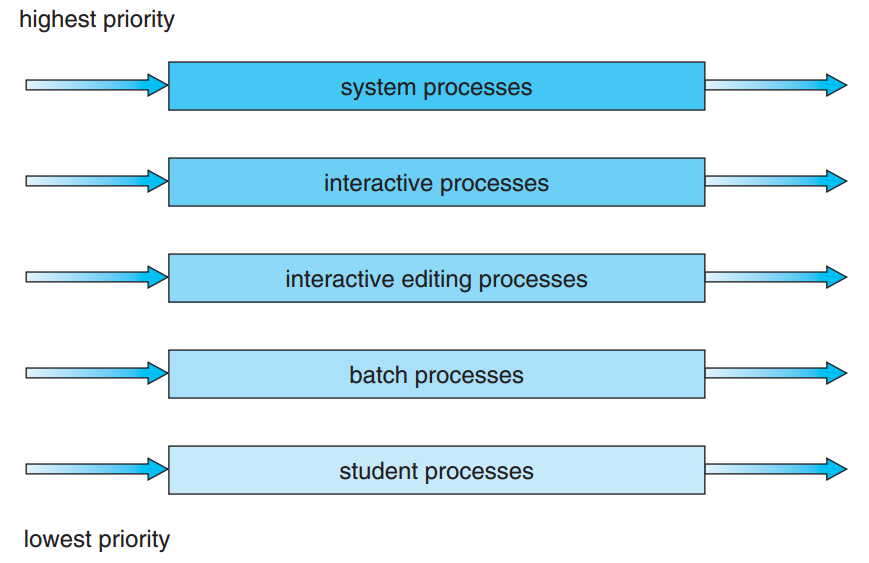
\includegraphics[width=1\textwidth]{img/mlq}
		\end{figure}
	\end{minipage}\hfill
\end{figure}
\end{frame}
%--------------------------------------------------------------------------------%


%--% Colas Multinivel con Retroalimentacion (MLFQ) %----------------------------------------------------%
\begin{frame}
\frametitle{\algTitle Colas Multinivel con Retroalimentacion (MLFQ)}

Parecido al MLQ, pero aqui los procesos no estan restringidos a quedarse en la cola en la que entraron,
pueden cambiar de una cola a otra.
Agrupa los procesos según las características de sus ráfagas de CPU.

\begin{figure}[h]
	\centering
	\begin{minipage}{0.60\textwidth}
		\centering
		\begin{itemize}
			\item \textbf{Ventajas}
			\begin{itemize}
				\item Es general y adaptable a cualquier sistema.
			\end{itemize}
			\vspace{0.5cm}
			
			\item \textbf{Desventajas}
			\begin{itemize}
				\item Es bastante complejo y costoso.
			\end{itemize}
		\end{itemize}
	\end{minipage}\hfill
	\begin{minipage}{0.40\textwidth}
		\centering
		\begin{figure}
			\centering
			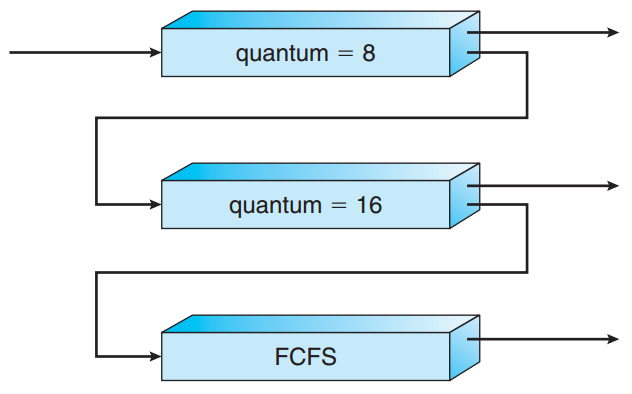
\includegraphics[width=1\textwidth]{img/mlfq}
		\end{figure}
	\end{minipage}\hfill
\end{figure}
\end{frame}
%--------------------------------------------------------------------------------%


%--% Sistemas de Tiempo Real %--------------------------------------------------%
\begin{frame}
\frametitle{Sistemas de Tiempo Real}

Los procesos deben terminar su ejecución en un periodo de tiempo
Estan los Soft Real-Time Systems y los Hard Real-Time Systems.

\begin{itemize}
	\item \textbf{Planificación de tablas estáticas}: Se conocen los procesos críticos a priori.
	
	\item \textbf{Planificación apropiativa con prioridad estática}: Cada proceso tiene una prioridad segun
	el tiempo en el que deben ser completados.
	
	\item \textbf{Planificación dinámica}: Hace un plan de ejecución con la información de los procesos.
	
	\item \textbf{Dynamic best-effort}: El sistema hace lo que puede por cumplir los tiempos propuestos. Los procesos
	podrian ser abortados.
\end{itemize}
\end{frame}
%--------------------------------------------------------------------------------%


%--% Planificación para Linux %--------------------------------------------------%
\begin{frame}
\frametitle{Planificación para Linux}

\begin{itemize}
	\item Usa un algoritmo basado en prioridades y apropiativo.
	\item Algoritmo de planificación que corre en tiempo \bigO{1} sin importar 
	el numero de procesos.
	\item El kernel mantiene una lista de todas las tareas ejecutables en una estructura de datos denominada cola de ejecución,
	y cada cola tiene 2 matrices de prioridades (Activa y Caducada).
\end{itemize}
\vspace{0.5cm}

\begin{figure}[h]
	\centering
	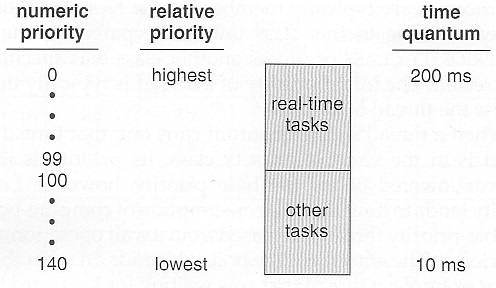
\includegraphics[width=0.5\textwidth]{img/5_15_PrioritiesVS_Length}
	\caption{\label{img:linux1}Relación entre prioridades y el tiempo dedicado que poseen.}
\end{figure}
\end{frame}
%--------------------------------------------------------------------------------%


%--% Planificación para Windows %------------------------------------------------%
\begin{frame}
\frametitle{Planificación para Windows}

\begin{itemize}
	\item Usa un algoritmo apropiativo basado en prioridades.
	\item Existe un hilo especial ``Idle'' que se ejecuta cuando ningún otro hilo esta listo.
	\item Existe una relación entre las prioridades del kernel de Windows y el API de Windows.
	\item A cada proceso se le da una prioridad base dentro de su clase de prioridad.
	\item A los procesos en primer plano se les multiplica su quantum de tiempo planificado
	por 3, para que tengan mejor respuesta.
\end{itemize}
\end{frame}
%--------------------------------------------------------------------------------%


%--% Planificación en sistemas Multiprocesadores %------------------------------------------------%
\begin{frame}
	\frametitle{Planificación en sistemas Multiprocesadores}
	
	La planificación se complica porque ahora hay mas de un CPU al que se debe tener ocupado y en uso
	efectivo de manera constante.
	
	\begin{itemize}
		\item Compartir la carga ayuda ya que balancea el trabajo entre múltiples procesadores.
		\item Si los CPU son distintos cada uno tiene su propia cola y algoritmo de planificación.
		\item Si los CPU son iguales, uno toma el papel de master y corre todo el codigo del kernel
		y controla todas las actividades, mientras que los demas corren codigo de usuario.
	\end{itemize}
\end{frame}
%--------------------------------------------------------------------------------%


%--% Planificación en sistemas Multicore %------------------------------------------------%
\begin{frame}
	\frametitle{Planificación en sistemas Multicore}
	
	\begin{itemize}
		\item Mejoras en el consuma de energía.
		\item Varios procesadores en un solo chip físico.
		\item El sistema operativo siguen siendo multiples procesadores.
	\end{itemize}
\end{frame}
%--------------------------------------------------------------------------------%


%--% Planificación de hilos %------------------------------------------------%
\begin{frame}
	\frametitle{Planificación de hilos}
	
	\begin{itemize}
		\item El sistema operativos planifica los hilos a nivel de kernel, los
		hilos a nivel de usuario son gestionados por una librería de hilos y el kernel no es consciente
		de ellos.
		\item Los hilos de usuarios deben ser asignados a un hilo de nivel
		de kernel asociado.
		\item La biblioteca de hilos planifica los hilos de usuario para que se ejecuten sobre proceso LWP disponible.
		\item El kernel usa el ámbito de contienda del sistema (SCS, system contention scope), para decidir que hilo del kernel planificar en un CPU.
	\end{itemize}
\end{frame}
%--------------------------------------------------------------------------------%


%--% Criterios para evaluar los algoritmos %-------------------------------------%
\begin{frame}
\frametitle{Criterios para evaluar los algoritmos}

\begin{itemize}
	\item \textbf{Modelado determinista}:
	\begin{itemize}
		\item Evaluación analítica.
		\item Define el rendimiento de cada algoritmo para una carga de trabajo predeterminada.
		\item Es simple y rápido.
	\end{itemize}
	\vspace{0.5cm}
	
	\item \textbf{Modelado de colas}:
	\begin{itemize}
		\item Evaluación analítica.
		\item Los resultados suelen ser cuestionables.
		\item Los análisis pueden plantearse matemáticamente, pero no se apegan a la realidad.
	\end{itemize}
\end{itemize}
\end{frame}

\begin{frame}
	\frametitle{Criterios para evaluar los algoritmos}
	
	\begin{itemize}
		\item \textbf{Simulación}:
		\begin{itemize}
			\item Gran precisión.
			\item Requieren recopilar o generar información para ejecutar la simulación.
			\item En la mayoría de los casos requieren mucho tiempo.
			\item Mientras mas larga, mas precisa pero requiere mas tiempo de computo.
		\end{itemize}
		\vspace{0.5cm}
		
		\item \textbf{Implementación}:
		\begin{itemize}
			\item Es el criterio con mayor precisión.
			\item Alto coste para su implantación.
		\end{itemize}
	\end{itemize}
\end{frame}
%--------------------------------------------------------------------------------%


\end{document}